\begin{figure}[htb]
    \centering
    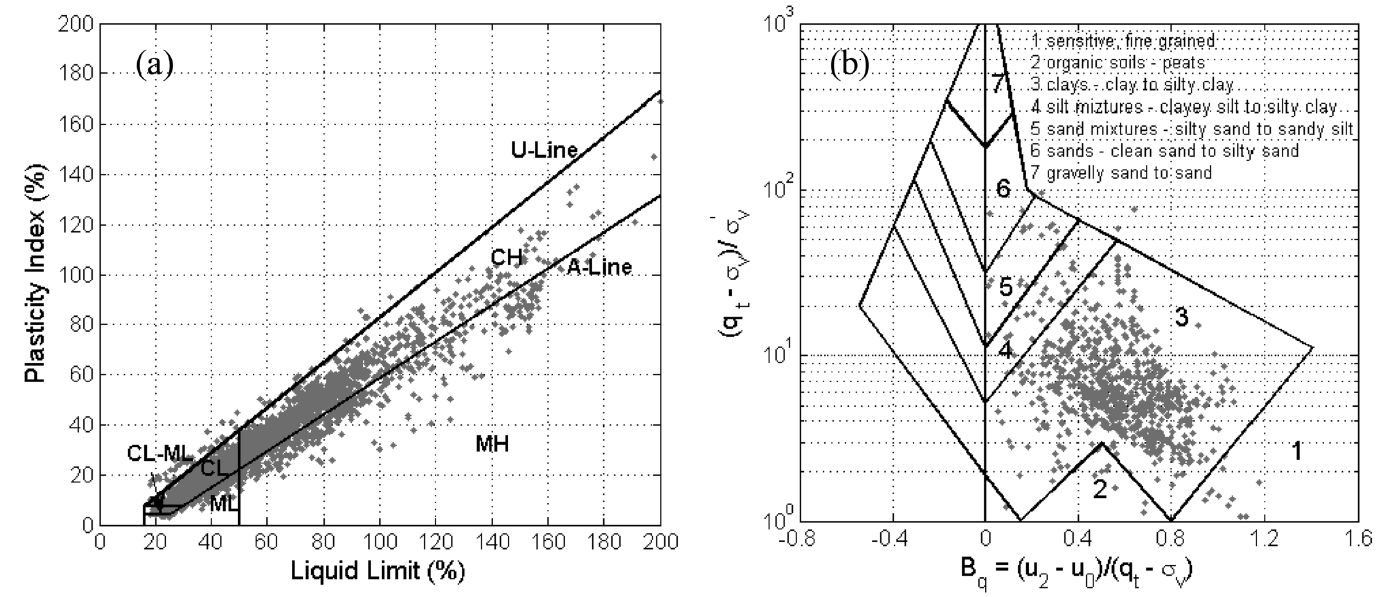
\includegraphics[width=0.8\textwidth]{figures/figure-1.png}
    \caption{(a) Plasticity chart; (b) \citet{Robertson1990151} CPTU soil classification chart. $B_q$, pore pressure ratio; CH, high-plasticity clay; CL, lowplasticity clay; MH, high-plasticity silt; ML, low-plasticity silt; $q_t$, corrected cone tip resistance; $u_0$, hydrostatic pore pressure; $u_2$, pore pressure behind the cone; $\sigma_v$, total effective stress; $\sigma_v'$, vertical effective stress.}
    \addtocounter{figure}{-1}
    \vspace{-5pt}
    \renewcommand{\figurename}{图}
    \caption{(a)可塑性图; (b)\citet{Robertson1990151}的CPTU土壤分类图。 $B_q$,孔隙压力比; CH,高塑性粘土; CL,低塑性粘土; MH,高塑性淤泥; ML,低塑性淤泥; $q_t$,校正的锥头电阻; $u_0$,静水孔隙压力; $u_2$,锥体后面的孔隙压力; $\sigma_v$,总有效应力; $\sigma_v'$,垂直有效应力。}
    \renewcommand{\figurename}{Figure}
    \label{figure:1}
\end{figure}